\documentclass[20pt,a4paper,oneside]{article}
\usepackage[utf8]{inputenc}
\usepackage[T1]{fontenc}
\usepackage[italian]{babel}
\usepackage{geometry}
\usepackage{graphicx}
\usepackage{sectsty}
\usepackage{mathtools}
\usepackage{tocloft}
\usepackage{verbatim}

\sectionfont{\fontsize{25}{30}\selectfont}

\geometry{top=3cm}
\geometry{bottom=3cm}
\geometry{left=2.5cm}
\geometry{right=2.5cm}
\linespread{1.2}

\title{\center 
\includegraphics[width=4cm]{logo_UniME}\\
\textsc{\huge{Università degli studi di messina}}\\
\textsc{\Large{Dipartimento di Matematica e Informatica}}\\[2cm]
\textbf{\Huge{Progetto Sistemi Operativi}\\
\huge{Simulatore per l'allocazione dei processi}\\
\large{Anno Accademico 2014-15}}}

\author{ a cura di\Large{ Davide Iuffrida }}

\date{}

\renewcommand{\cfttoctitlefont}{\fontsize{30}{10}\selectfont\bfseries}

\renewcommand\cftsecfont{\fontsize{12}{8}\selectfont\bfseries}

\begin{document}
\maketitle
\newpage
\pagenumbering{Roman}
\tableofcontents
\newpage
\pagenumbering{arabic}

\fontsize{14}{14}\selectfont

\section{Introduzione}
È richiesta l'implementazione di un applicativo che simuli tre delle tecniche usate per eseguire l'allocazione
della memoria utilizzando una free-list: \\
\textbf{First-Fit}, \textbf{Best-Fit} e \textbf{Worst-Fit}. \par
L'applicativo deve prevedere una situazione iniziale (randomica) della memoria e confrontare il risultato finale
ottenuto dalle tre teniche. \par
È richiesto inoltre che ogni confronto costi una unità, e che vengano analizzate le differenze delle tre tecniche
in termini di costo e in termini di frammentazione esterna. L'applicativo dovrà, inoltre, prevedere i boundary tag
per facilitare l'uso delle aree di memoria libere.\par
È anche richiesto che il \textbf{numero di simulazioni} da effettuare sia dato
in input. L'applicativo dovrà effettuare le simulazioni al fine da esaminare il diverso comportamento delle tre tecniche
mostrando ad ogni simulazione lo stato del sistema sia a video che su file di log. \par

\section{Allocazione dei processi}
In un sistema operativo, quando dev'essere eseguito un software, questo verrà caricato sulla memoria centrale dalla memoria secondaria. Un software, quando viene eseguito, viene definito come processo. Il sistema operativo, mantiene una lista dei processi che sono attivi in memoia, e, attraverso uno scheduler, inserisce man mano nuovi processi in esecuzione prelevandoli dalla lista dei processi pronti. Quando un processo dev'essere allocato, potremo utilizzare diversi algoritmi. I più utilizzati sono:

\begin{itemize}

\item \textbf{First-Fit}: L'allocatore sceglierà il primo blocco disponibile che potrà contenere il nostro processo.
\item \textbf{Best-Fit}: L'allocatore sceglierà il blocco libero più piccolo che possa contenere il processo.
\item \textbf{Worst-Fit}: L'allocatore sceglierà il blocco libero più grande che possa contenere il processo.

\end{itemize}

Una volta che un blocco viene scelto, questo verrà rimosso dalla freelist, ed assegnato al processo, fino a quando questo non finirà la sua esecuzione. Una volta che la sua esecuzione è terminata, questo rilascerà la memoria occupata, e verrà reinserito il blocco nella freelist. \newpage
Tramite l'utilizzo della tecnica di Boundary Tag, terremo un riferimento al blocco precedente e successivo, in modo che se due blocchi, sono vicini tra loro ed entrambi liberi, allora potremo unirli in un unico blocco.

ver\section{Implementazione dell'applicativo}
L'applicazione è stata realizzata con il linguaggio \textbf{Python}, utilizzando la versione \textbf{2.7}.\par
Il codice è stato ottimizzato e reso riutilizzabile grazie all'uso delle classi. \par
Le funzionalità dell'applicazione sono state divise in diverse classi:
\begin{itemize}
\item \textbf{Memory}: questa classe gestirà la nostra memoria, fornendo i metodi per poter gestire la freelist ed i vari blocchi
che formano la memoria. Conterrà la \textbf{grandezza della memoria}, una lista ai vari \textbf{blocchi di memoria} che formano la memoria,
una lista per la \textbf{freelist}, una lista dei \textbf{processi} attivi sulla memoria al momento, ed un riferimento al \textbf{logger}.

\item \textbf{MemoryBlock}: questa classe gestirà i nostri blocchi di memoria, con informazioni riguardo al \textbf{valore iniziale} ed il \textbf{valore finale} del blocco,
la \textbf{dimensione} totale di questo blocco, e lo stato (se è al momento allocato o meno). Verrà fornito un metodo per l'aggiornamento della dimensione
del blocco.

\item \textbf{Process}: questa classe gestirà le informazioni riguardo ai processi, tra cui la \textbf{dimensione} che il processo richiede, un \textbf{tempo di inizio} che equivale al tempo in cui il processo entrerà in esecuzione, il \textbf{blocco} in cui è stato allocato il processo, ed il \textbf{tempo di lavoro} richiesto per completare il suo lavoro.

\item \textbf{AllocationManager}: questa classe è il fulcro che permette all'applicazione di eseguire i diversi algoritmi. Conterrà le informazioni riguardo alla \textbf{memoria} su cui andrà a lavorare, una lista dei \textbf{processi in attesa} di essere eseguiti ed un riferimento al logger. Avrà diversi metodi, tra cui quelli che serviranno a compiere le allocazioni. Abbiamo il metodo per il \textbf{First-Fit}, tramite la quale allocheremo i processi nel primo blocco libero che può contenere il nostro processo; il \textbf{Best-Fit}, che cercherà di allocare il processo in un blocco che, tra tutti, abbia una dimensione molto più vicina a quella del processo; infine abbiamo il \textbf{Worst-Fit}, tramite la quale allocheremo il processo cercando il blocco più grande tra quelli liberi. Abbiamo altri metodi che verranno usati come supporto dagli algoritmi, come il \textbf{clearMemory} che verrà avviato all'inizio di ogni istante di tempo di vita dell'algoritmo, e pulirà la memoria da processi che hanno terminato la loro attività. Il metodo \textbf{checkForProcesses} ci restituirà un processo che corrisponderà al nostro istante di tempo, in modo da poterlo mandare in esecuzione. Uno dei più importanti è l'\textbf{allocateProcess}, che allocherà il processo in attesa nel blocco di memoria indicato. Il metodo \textbf{isMemoryAllocated} ci dirà se almeno un blocco di memoria è allocato. Per ultimo, troviamo \textbf{graphicStateOfMemory}, nella quale stamperemo una versione grafica dello stato della memoria per ogni istante di tempo, indicando la dimensione del blocco di memoria, e, tramite due lettere di riferimento (T: Allocato, F: Non Allocato), ci indicherà i blocchi liberi da quelli pieni.
\end{itemize}
Abbiamo inoltre altre due classi che utilizziamo per facilitare il print del nostro applicativo, e per gestire i colori che vengono applicati sulla shell, che sono \textbf{Log} e \textbf{Colors}. La classe Log verrà inizializzata per stampare su due diversi file, uno chiamato log.txt e l'altro log\_colored.txt, nella quale verranno stampate le simulazioni, ed in cui in log\_colored.txt salveremo anche i caratteri di escape per i colori, in modo da poterlo visualizzare in un secondo momento sulla shell tramite il comando "\textbf{cat}". \par
Nella parte principale del programma, verrà fatto innanzitutto un controllo se il nostro applicativo è stato avviato passando per argomento il numero di simulazioni, altrimenti verrà richiesto l'input da tastiera. Verranno inizializzate tutte le variabili per quanto riguarda le informazioni sulla memoria, dimensione dei processi, etc... Dopodiché inizierà un ciclo che continuerà per il numero di simulazioni scelto. \par
Ogni qualvolta che inizia una nuova simulazione, verrà inizializzata la memoria, e verranno ricreati i processi che dovranno essere allocato in memoria, a cui verranno attribuiti i valori randomici allle informazioni descritte sopra, quando parlavamo della descrizione della classe che definisce i processi. \par
Dopodiché inizieremo ad effettuare i nostri algoritmi, però prima creeremo delle copie locali della nostra memoria e dei nostri processi, in modo che i tre algoritmi possano funzionare sulla stessa identica situazione, ed avere un confronto migliore. Ogni qualvolta che un algoritmo finirà la sua esecuzione restituirà dei valori, che verranno usati a calcolare le statistiche finali. Una volta che le simulazioni saranno finite, il programma terminerà stampando quelle che sono stati i risultati da lui ottenuti. 
\newpage
Le statistiche che vengono effettuate sono:

\begin{itemize}

\item \textbf{Media della dimensione dei blocchi liberi}, in cui calcoleremo la dimensione media che avremo alla conclusione dell'esecuzione di un algoritmo.
\item \textbf{Media sui confronti effettuati}, che varierà a seconda delle volte che l'algoritmo ha dovuto confrontare il processo con i blocchi liberi per poter provare ad effettuare un allocazione.
\item \textbf{Media delle allocazioni fallite}, queste avvengono nel caso in cui il processo non può essere inserito in nessun blocco libero per la loro piccola dimensione. Inoltre, verrà anche conteggiato quanti di questi fallimenti siano per frammentazione esterna, e cioè, quante di queste volte, l'unione di tutti i blocchi liberi, avrebbe portato ad un blocco unico che sarebbe bastato a tenere il processo in memoria.
\item \textbf{Media di frammentazione esterna}, questo valore è calcolato tramite la seguente formula: 
\begin{equation*}
Frammentazione Esterna = 1 - \frac{Blocco Libero Piu Grande}{Memoria Libera Totale}
\end{equation*}
Questo calcolo verrà effettuato ogni qualvolta verrà trovata una frammentazione esterna, e ne verrà fatta la media tra tutte le simulazioni.

\end{itemize}

Le statistiche che invece potremo visualizzare alla fine di ogni algoritmo sono:

\begin{itemize}
\item \textbf{Numero di confronti}, i confronti che vengono fatti dall'algoritmo in quella singola sessione.
\item \textbf{Allocazioni fallite}, un contatore delle allocazioni fallite, di cui vengono contate anche quelle per \textbf{frammentazione esterna}.
\item \textbf{Frammentazione Esterna}, calcolo sulla frammentazione esterna riguardo all'intera esecuzione dell'algoritmo, utilizzando la stessa formula descritta precedentemente.
\end{itemize}

\newpage

\section{Diagramma UML delle classi}
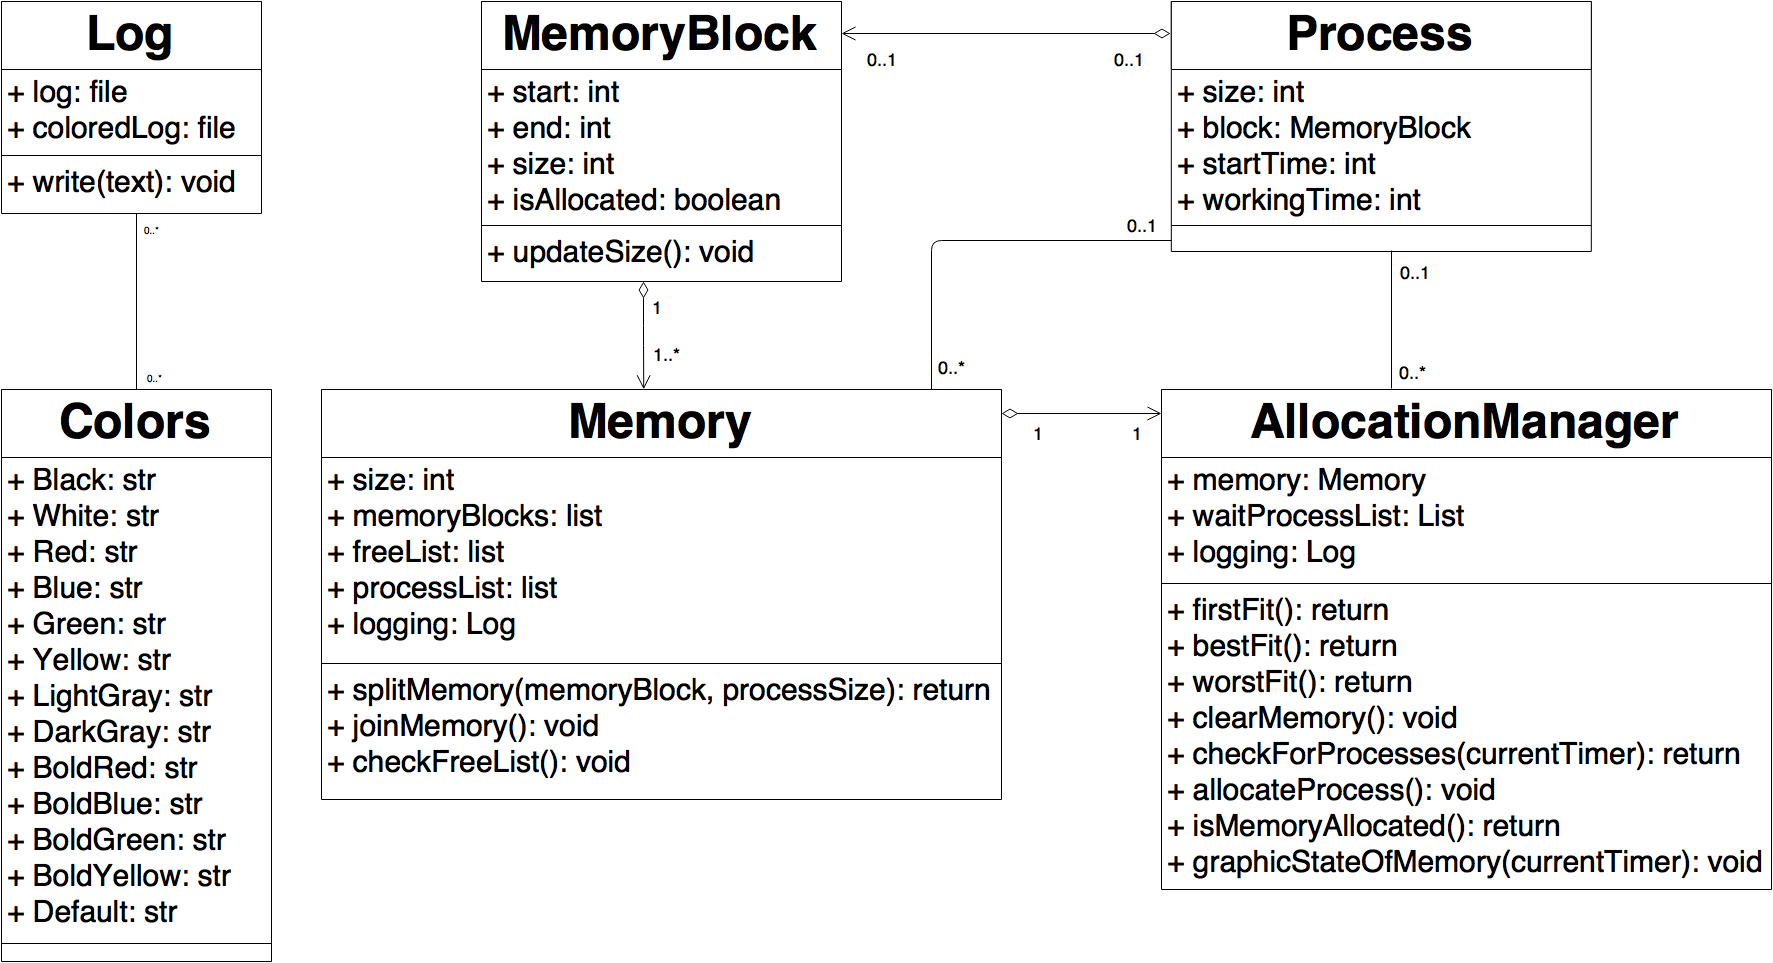
\includegraphics[scale=0.26]{ClassDiagram.png}

\newpage
\section{Diagrammi a blocchi}
Per primo, vediamo un esempio di diagramma a blocchi per quanto riguarda l'esecuzione del programma.\\
\begin{center}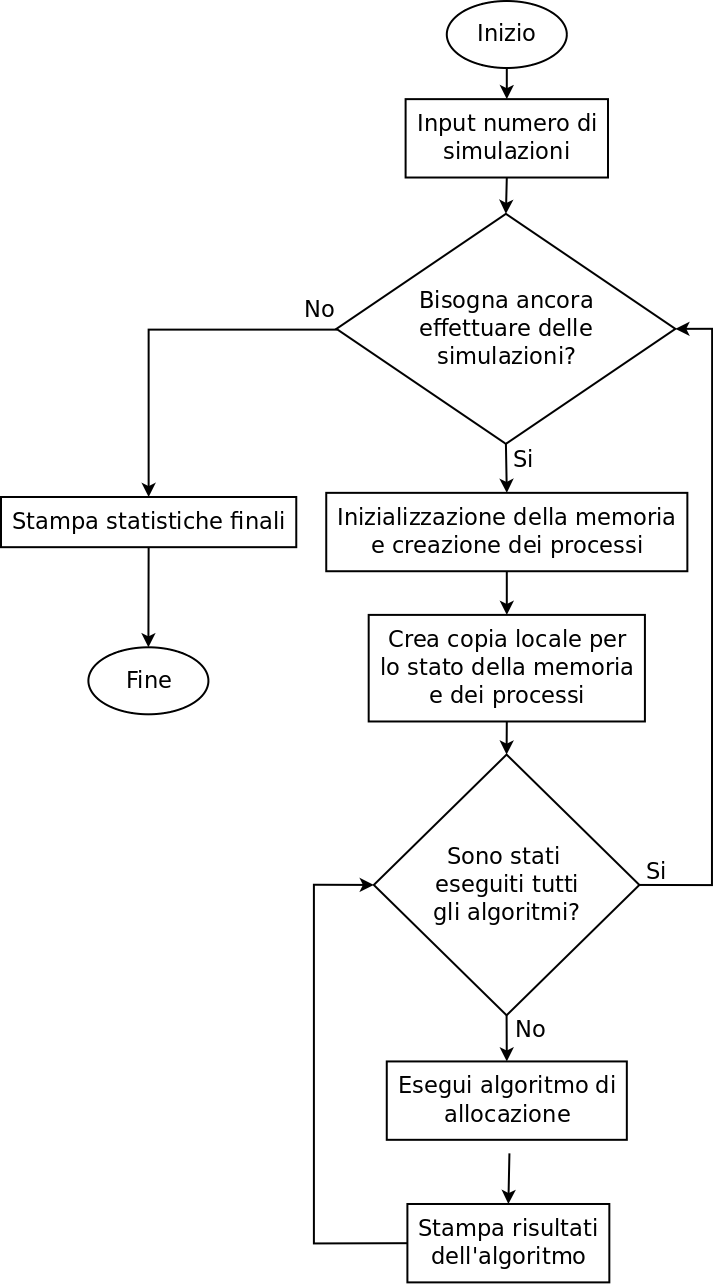
\includegraphics[scale=0.26]{AD1}\end{center}

\newpage

Qui di seguito troviamo un esempio di diagramma a blocchi per l'algoritmo d'allocazione dei processi \textbf{First-Fit}.\\
\begin{center}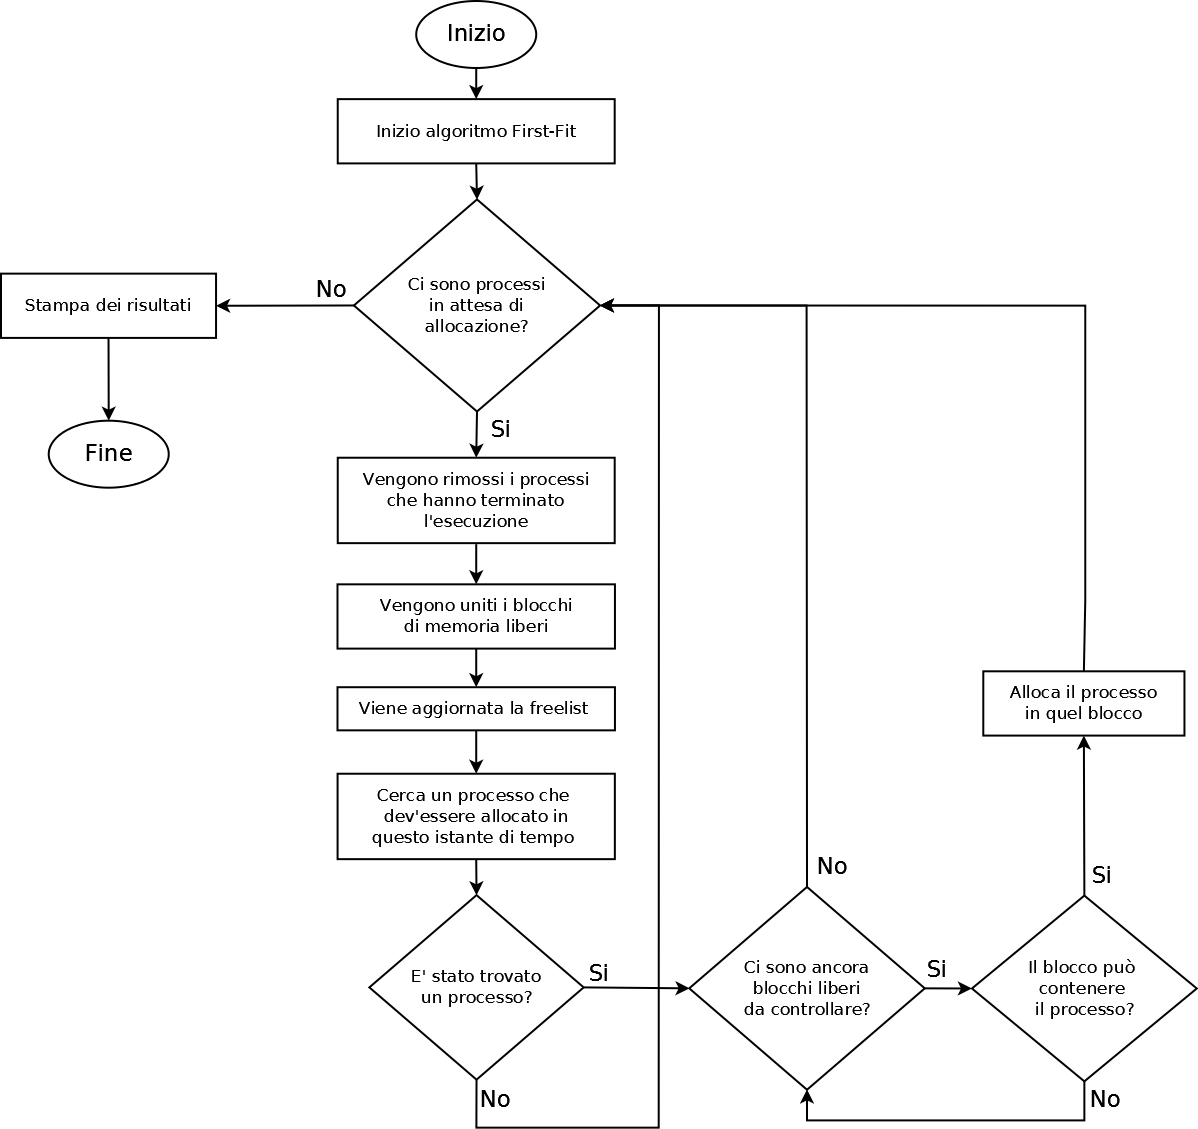
\includegraphics[scale=0.26]{AD2}\end{center}

\newpage

\section{Manuale d'uso}
Come detto già in precedenza, l'applicazione è stata scritta utilizzando Python \textbf{2.7}, quindi per essere eseguito richiederà questa stessa versione per avere una migliore compatibilità. Per avviare l'applicazione da terminale, bisognerà utilizzare il comando \textbf{python Process\_Allocator.py}, che potrà essere seguito da un valore numerico che indicherà il numero di simulazioni. \par
Nel caso in cui questo non venga inserito, sarà possibile inserirlo successivamente da input direttamente ad applicazione eseguita. Dopo che l'applicazione avrà completato tutte le simulazioni, creerà due file log nella stessa cartella in cui è contenuto il file .py, di cui uno manterrà i colori che appariranno anche in shell, per un futuro utilizzo tramite il comando \textbf{cat}, mentre l'altro avrà semplicemente il print del nostro applicativo, senza colori, e più comprensibile da un qualsiasi editor di testo. 

\newpage

\section{Conclusioni sui risultati ottenuti}
I seguenti risultati sono stati ottenuti su un numero di simulazioni pari a 1000, in modo da avere dei risultati più precisi su cui poter porre le nostre conclusioni sull'esperimento.
\begin{verbatim}
RISULTATI FINALI

Media dimensione blocchi liberi First-Fit: 3478
Media dimensione blocchi liberi Best-Fit: 3561
Media dimensione blocchi liberi Worst-Fit: 3540

Media confronti First-Fit: 78
Media confronti Best-Fit: 117
Media confronti Worst-Fit: 118

Numero di allocazioni fallite First-Fit: 2328, 
di cui 2059 per via della frammentazione esterna
Numero di allocazioni fallite Best-Fit: 2117, 
di cui 1834 per via della frammentazione esterna
Numero di allocazioni fallite Worst-Fit: 3110,
di cui 2872 per via della frammentazione esterna

Media di frammentazione esterna First-Fit (%): 27.81%
Media di frammentazione esterna Best-Fit (%): 25.37%
Media di frammentazione esterna Worst-Fit (%): 34.69%
\end{verbatim}

Prima di passare alle conclusioni però, dobbiamo dare spazio ad alcune informazioni riguardo al tempo d'esecuzione dei singoli algoritmi. Spesso, questi saranno gli stessi, però può accadere che, il fallimento dell'allocazione di un processo per mancanza di spazio / frammentazione esterna, può portare ad un aumento del tempo d'esecuzione per un processo rispetto ad un altro. Detto questo, possiamo quindi trarre le seguenti conclusioni riguardo ai singoli algoritmi:
\begin{itemize}
\item \textbf{First-Fit}: il First-Fit sembra essere il migliore algoritmo per un'allocazione molto rapida, visto che è l'algoritmo che necessita del minor numero di di confronti per poter allocare un blocco di memoria. Con l'allocazione dell'ultimo processo in memoria, il First-Fit avrà un minore spazio libero rimanente, e quindi che è riuscito ad allocare più processi in memoria contemporaneamente. Il First-Fit avrà un alto numero di fallimenti per le allocazioni, dovuto al fatto che, allocando i processi, si creeranno dei frammenti di memoria troppo piccoli per allocarne altri, e questo porterà spesso ad avere frammentazione esterna sulla memoria. Sul totale delle allocazioni fallite, nel nostro caso, il 27.81%, calcolato usando la formula specificata prima, cioè:\\
\begin{equation*}
Frammentazione Esterna = 1 - \frac{Blocco Libero Piu Grande}{Memoria Libera Totale}
\end{equation*}
\\
vedremo che sarà uno degli algoritmi a portare ad una maggiore frammentazione esterna.

\item \textbf{Best-Fit}: il Best-Fit, come velocità può essere quasi paragonato al Worst-Fit, però possiamo notare come la sua media sulla dimensione dei blocchi sia più alta rispetto al First, e quindi riuscirà ad allocare più processi assieme nel tempo, lasciando meno processi da allocare all'ultimo istante, lasciando più spazio libero. Ha una minore possibilità di fallire un'allocazione rispetto agli altri due algoritmi, poiché, prendendo i blocchi più piccoli per poter contenere un processo, questi lasceranno blocchi più grandi ad altri processi, che riusciranno a contenersi in maggior numero; la maggior parte delle allocazioni fallite saranno per frammentazione esterna. La media di frammentazione esterna, ci risulta quindi essere un valore più basso del First e Worst -Fit, infatti avremo un 25.37% in media, che è ottimo per un algoritmo di allocazione. Possiamo quindi dire che il Best-Fit non sarà ottimo a livello di velocità, ma per quanto riguarda la frammentazione, è sicuramente il migliore.

\item \textbf{Worst-Fit}: il Worst-Fit, risulta essere il peggiore sia in velocità che frammentazione. Avremo sempre un maggior numero di confronti rispetto agli algoritmi, anche se di poco più lento del Best-Fit; la dimensione media dei blocchi liberi sarà molto simile a quello degli altri algoritmi, quindi riguardo a questo aspetto, poco importa l'algoritmo utilizzato. Il Worst-Fit avrà un alto numero di allocazioni fallite, di cui molte per frammentazione estenra, per via dei blocchi molto più grandi che lascerà in memoria, che spesso potranno non essere abbastanza grandi da contenere un processo, e potrebbero restare in attesa per molto tempo se posizionato tra due processi con una lunga attività. La sua media di frammentazione esterna, sarà del 34.69% circa. Ovviamente, su qualsiasi punto di vista, risulta essere il peggior algoritmo da utilizzare.
\end{itemize}

Dopo aver tratto queste conclusioni, possiamo quindi affermare che First-Fit e Best-Fit sono i due algoritmi migliori, in cui, se si è alla ricerca di un algoritmo con una maggiore velocità, si sceglie First-Fit, altrimenti, se si cerca un algoritmo a bassa frammentazione esterna, sarà meglio l'utilizzo di Best-Fit. Visti i risultati, è ovviamente molto sconsigliato l'uso del Worst-Fit.


\end{document}